\documentclass[a4paper]{article}

\usepackage[pages=all, color=black, position={current page.south}, placement=bottom, scale=1, opacity=1, vshift=3mm]{background}
\SetBgContents{

}      % copyright

\usepackage[margin=1in]{geometry} % full-width

% AMS Packages
\usepackage{amsmath}
\usepackage{amsthm}
\usepackage{amssymb}
\usepackage{graphicx}
\usepackage{wrapfig}
% Unicode
\usepackage[utf8]{inputenc}
\usepackage{hyperref}
\hypersetup{
	unicode,
%	colorlinks,
%	breaklinks,
%	urlcolor=cyan, 
%	linkcolor=blue, 
	pdfauthor={Author One, Author Two, Author Three},
	pdftitle={A simple article template},
	pdfsubject={A simple article template},
	pdfkeywords={article, template, simple},
	pdfproducer={LaTeX},
	pdfcreator={pdflatex}
}

% Vietnamese
%\usepackage{vntex}

% Natbib
\usepackage[sort&compress,numbers,square]{natbib}
\bibliographystyle{mplainnat}

% Theorem, Lemma, etc
\theoremstyle{plain}
\newtheorem{theorem}{Theorem}
\newtheorem{corollary}[theorem]{Corollary}
\newtheorem{lemma}[theorem]{Lemma}
\newtheorem{claim}{Claim}[theorem]
\newtheorem{axiom}[theorem]{Axiom}
\newtheorem{conjecture}[theorem]{Conjecture}
\newtheorem{fact}[theorem]{Fact}
\newtheorem{hypothesis}[theorem]{Hypothesis}
\newtheorem{assumption}[theorem]{Assumption}
\newtheorem{proposition}[theorem]{Proposition}
\newtheorem{criterion}[theorem]{Criterion}
\theoremstyle{definition}
\newtheorem{definition}[theorem]{Definition}
\newtheorem{example}[theorem]{Example}
\newtheorem{remark}[theorem]{Remark}
\newtheorem{problem}[theorem]{Problem}
\newtheorem{principle}[theorem]{Principle}

\usepackage{graphicx, color}
\graphicspath{{fig/}}

%\usepackage[linesnumbered,ruled,vlined,commentsnumbered]{algorithm2e} % use algorithm2e for typesetting algorithms
\usepackage{algorithm, algpseudocode} % use algorithm and algorithmicx for typesetting algorithms
\usepackage{mathrsfs} % for \mathscr command

\usepackage{lipsum}
% Author info





\begin{document}
\begin{titlepage}
    \centering
     {
\includegraphics[width=0.2\textwidth]{logo}\par}
    {\bfseries\LARGE Universidad Castilla La Mancha\par}
    \vspace{1cm}
    {\scshape\Large Escuela Superior Informática\par}
    \vspace{2cm}
    {\scshape\Huge Translation \par}
    {\itshape\Large Intelligent Systems - Take home assigment \par}
    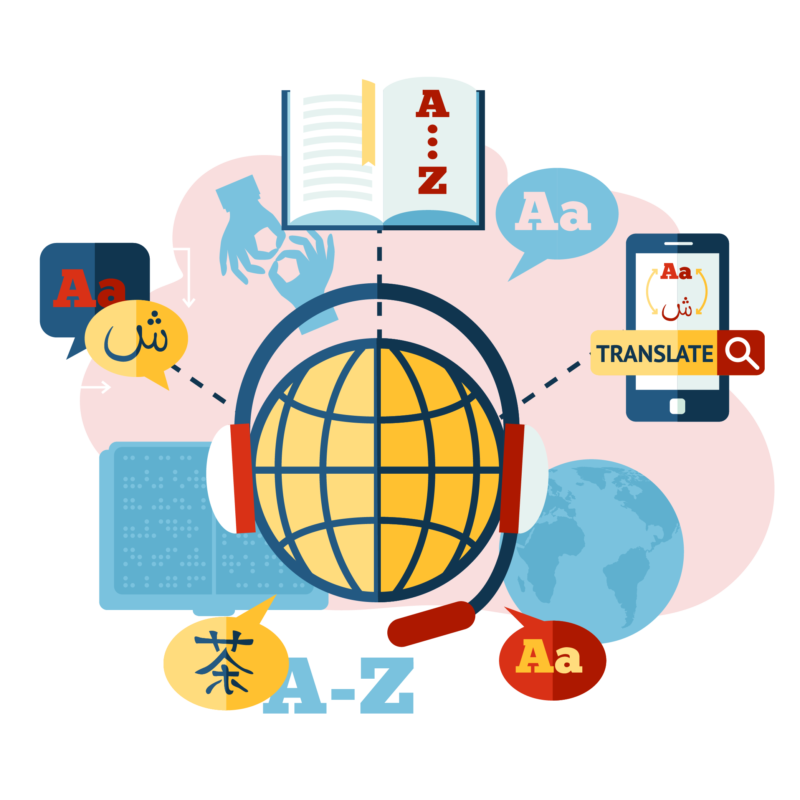
\includegraphics[width=0.7\textwidth]{INTERPRETACION-O1-800x800.png}
    \vfill
    {\Large Author: \par}
    {\Large María Jesús Dueñas Recuero\par}
    \vfill
    {\Large November 2021 \par}
    
   
\end{titlepage}
\begin{abstract}
    Given the increase in globalisation, every day we are in contact with a greater number of cultures, which forces us, in a healthy way, to learn new languages.\newline

	However, thanks to the development of technology and artificial intelligence, it is not necessarily necessary to study a language for years in order to understand it, given that translator websites and the translators themselves allow us to interact with it fluently.\newline

	It is an opportunity to broaden our knowledge and understanding of other languages. As well as guaranteeing the correct use of the language for work and business, as they not only translate a language but also interpret emotions and feelings.
\end{abstract}

	\newpage
	
	\tableofcontents
	\newpage
	\section{Introduction}
	\label{sec:intro}
	Artificial intelligence (AI) technology is changing the way people go about their daily lives, not only enabling them to read in their native language, but also to read in different languages and understand them perfectly, and even to be aware of the sentimentality of the text thanks to machine translation.\newline

    Professionals are aware of the importance of AI in the development of machine translation, however, there are still many barriers in this field as will be seen throughout the paper.


	
	
    
	
	


	
	
	\section{First approaches}
	\label{sec:examples}
    In the early years, around 1949,\textbf{Warren Weaver}  of the Rockefeller Foundation set up a cryptographic and language processing machine that was a precursor to the concept of machine translation. This project can be found in his \textbf{"Memorandum on Translation"}.\newline
    
    In 1954 the founding research team of the \textbf{Georgetown-IBM experiment} conducted a demonstration with a machine that could \textbf{translate 250 words} from Russian into English.\newline
    
    With this breakthrough people thought that machine translation would soon solve numerous problems and many translators began to fear for their jobs. However, the human brain is better able than a computer to access the complex framework of meaning, interpretation and syntax. In 1964,\textbf{the Automatic Language Processing Advisory Committee}  (ALPAC) declared that further investment in machine translation was not worthwhile.\newline
    
    During the 1970s and 1990s Canada, not thinking like ALPAC, and developed the \textbf{METEO system,} which translated weather reports from English into French, capable of translating 80,000 words a day and was such a success that it was used until the first half of the 21st century.\newline
    
    The 1980s saw the development of translation memory technology, which was the beginning of overcoming the challenge posed by the nuances of verbal communication, but systems continued to face the same challenges in trying to convert a text into another language without losing its meaning.\newline
    
    It was in 2000 when \textbf{Franz Josef Och}, a computer scientist, won the machine translation competition that he went on to become Google's Director of Translation Development. In 2012, Google announced its own translation app, Google translate. In addition, Japan is also leading the machine translation revolution with the creation of voice translations for mobile phones, which work in English, Japanese and Chinese. This is the result of the development of computer systems with a neural network model, rather than memory-based functions.\newline
    
    That is why in 2016, Google informed the public that the application of a \textbf{neural network technology }would improve the clarity of its translator, eliminating many of its errors. Called \textbf{Google Neural Machine Translation} (NLT), it began translating language combinations that it had not been taught, for example, programmers taught it to translate from English to Portuguese and Spanish, and it began translating from Portuguese to Spanish without assigning it that combination.
    
    
    

    \section{Main milestones}
	\label{sec:examples}
	Machine translation is a major research topic in the academic world, and several research groups are exploring various strategies, from those based on \textbf{inter-language} (EU Molto Project) to transfer rule-based systems such as Apertium, to purely \textbf{statistical systems} such as Moses.\newline

    In research, they try to establish links between translators and machine translation. These include those aimed at assessing the quality of machine translation and its impact on the productivity of professional translators.\newline

    Currently, we can speak of three types of automatic translation: the one using \textbf{linguistic information}, \textbf{the statistical} one and the one based on \textbf{neuronal networks}. 

    \subsection{Rule based machine translation}
    This type of machine translation is not more prevalent in research because it requires a large investment of time and resources. Because developing a single language pair requires source and target language grammars, as well as bilingual dictionaries and transfer rules. In addition, the system cannot translate linguistic structures that are not included in its grammars or transfer rules, nor words or expressions that are not in its dictionaries.\newline

    Rule-based engines must be practically continuous to ensure that they are able to translate texts from a new domain or grammatical structures that were not foreseen in the first place. \newline

    Although rule-based machine translation is not predominant in the academic world, its usefulness may go far beyond what we imagine, and it can be useful for language pairs where there is insufficient data to train other engines. Apertium, an open source platform for developing a translation engine, is a great catalyst for the development of minority language engines.
    
    \subsection{Statistical machine translation}
	As an alternative to the above process, statistical machine translators can be used which only need data to be trained. Specifically, they need as large a \textbf{monolingual corpus} of the target language as possible and a \textbf{parallel corpus} with translations between source and target language. This system consists of three components: 
    \begin{itemize}
        \item \textbf{The language model} is in charge of calculating the probability that a sentence in my target language is correct. It is in charge of translation fluency and is trained using a monolingual corpus of the target language that is as complete as possible.
         \item \textbf{The translation model} is responsible for establishing the correspondence between source and target language and is trained using a corpus aligned to the sentence level. In this phase, the translation probability is estimated from translations appearing in the training corpus.
         \item \textbf{The decoder} is in charge of searching among all the translations for the most appropriate one in each case.
    \end{itemize}
    The quality of these engines depends on many factors: the language pair used, the quality of the training corpus, the field, etc. However, the main reference for these systems is \textbf{Moses}, an open source machine translation system developed thanks to several European research projects with collaborations from all over the world.
    
    \subsection{Machine translation based on neural networks}
	
	This type of translation began to be heard about 2014 and was developed in the following years, however, in 1997 is the first time that this process was proposed but did not go ahead due to the limitation and the need for powerful computers and processors.\newline

         

    Nowadays, many research centres have access to supercomputers and this has encouraged their research, as well as the great advances that have been achieved. In 2016, these engines were the winners in the annual academic competitions.\newline
        
     
    They work as follows: these networks aim to emulate the way neurons in our brains work, in the same way that our neurons receive information and make connections with each other, the components of language associate with other underlying information to form associations and generate translations. In this way, using machine learning techniques, the computer learns to translate from large amounts of parallel text that also includes all kinds of linguistic and emotional information.\newline
     
    \newline
    Thanks to the way it relates the information associated with each word and that of the words in a sentence, the computer is able to learn to translate more efficiently.\newline
    \begin{figure}[h]
        \centering
        
        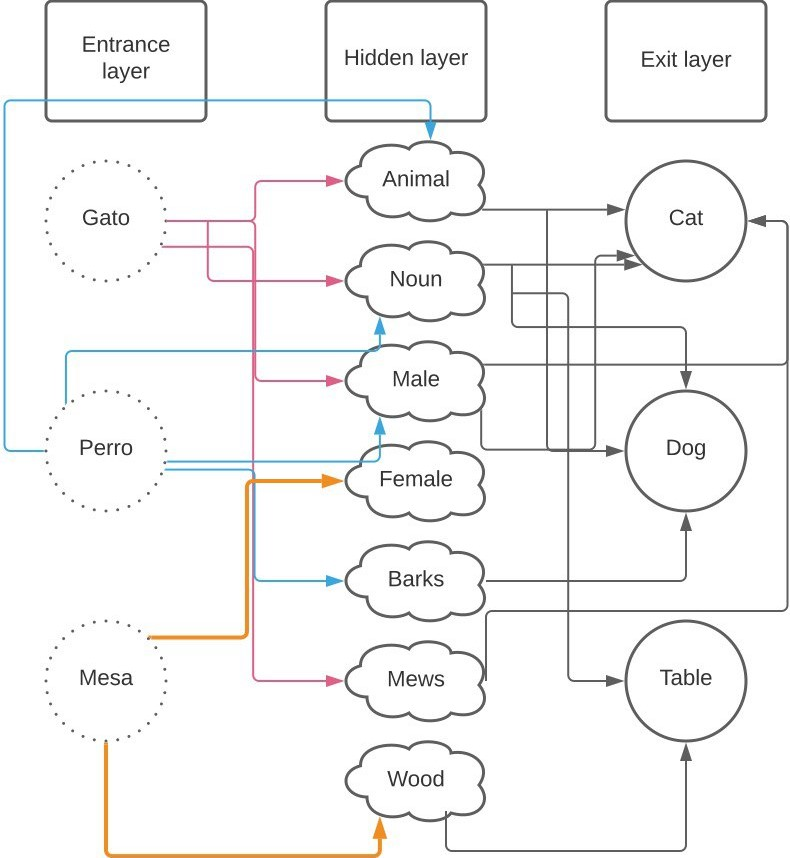
\includegraphics[width=0.4\textwidth]{neuronal.jpeg}
        \caption{Neuronal network translation from Spanish to English}
    \end{figure}
   
	Thus, using artificial neural networks, the system can learn that the terms ''dog'' and ''cat'' are more similar to each other than ''dog'' and ''table''.\newline


    The potential of machine translation based on neural networks is such that engines are already being trained that, in addition to text, incorporate images or even multimedia files.
    
    
    
    

	\section{Current status}
	Machine translation research is very active internationally, both in terms of the number of groups involved and the activity in conferences, workshops and associations. The IAMT sponsors  a list of translation software and resources organised by software type and vendor. It also organises a biannual conference on machine translation: which brings together the three affiliated associations. Research groups on machine translation are numerous. Sometimes it is a line of research within a research group covering different topics in natural language processing, sometimes machine translation is the main focus of research.\newline
	
	Some of the most significant translation projects are:

   \begin{flushleft}
    \textbf{Pattern Recognition and Human Language Technology (PRHLT) research group, Polytechnic University of Valencia}
   \end{flushleft}
    It investigates several areas, one of them being automatic translation of both text and spoken speech for restricted domains, based on statistics.the group has extensive experience in automatic speech recognition.the group has developed a large number of projects, a small sample of which are the following:
     \begin{itemize}
         \item Development of Statistical Techniques for Adaptive and Interactive Learning in Computer-Assisted Translation.
         \item Translation support based on translation memories.
        \item \textbf{SISHITRA:} hybrid systems for Valencian-Spanish translation from speech and text.
        \item \textbf{TRACOM: }Translation and Understanding of Spoken Language through Exemplar-based Learning Techniques.
    \end{itemize}
   

   \begin{flushleft}
    \textbf{TALP, Centre for Language and Speech Technologies and Applications of the Polytechnic University of Cataluña}
   \end{flushleft}
    They are developing their own \textbf{statistical speech translation system}, incorporating linguistic knowledge (morphological, syntactic and semantic) to improve its performance. The working languages are Spanish, Catalan and English, but also mandarin and Arabic. All this, in the framework of national and European projects. They are currently participating in the European project \textbf{MOLTO}, for a tool to translate texts between multiple languages instantly and with high quality, based on interlingua. Projects to be highlighted:
    \begin{itemize}
        \item \textbf{EuroOpenTrad: }open source machine translation for the European integration of the languages of the Spanish State. The translation system is available at http://www.opentrad.org/.
        \item\textbf{OpenTrad: }open source machine translation for the languages of the Spanish State.
        \item \textbf{MOLTO: }Multilingual Online Translation, funded by the European Union.
    \end{itemize}

	\label{sec:examples}
	\section{Future challenges}
	\label{sec:examples}

	In the future, machine translation will seek to design a content strategy and make decisions regarding which markets to pursue, making sure to take into account the highest possible efficiency in modern machine translation and related technologies.\newline

    In addition, it will seek to use \textbf{neural networks} to not only carry out a literal translation of content but also an interpretation of it, allowing it to not only translate technical texts but also to carry out translations in real time, such as during a conversation if necessary.\newline

    On the other hand, partnering with language service providers will help them implement translation to achieve the desired results, as well as improve their content and develop their marketing strategy. The enhancement of these features will allow:
    \begin{itemize}
        \item The ability to distribute content to the market more quickly
        \item Consistency of terminology
        \item Increased translator productivity
        \item Lower translation costs
    \end{itemize}
   
In addition to the above-mentioned scientific and technical research, artificial intelligence could recreate voices in other languages from the original one. The production of highly sophisticated digital voice is getting closer and closer every day. Entertainment and dubbing companies are already preparing for a revolution in the sound of series and films. It involves using artificial intelligence to \textbf{create human voices} from a live actor's voice sample, models that not only sound like the performers, but can speak any language, shout, laugh and even talk with their mouths full.\newline

In this way, with just a few samples, an entire language could be recreated with the original voice, and at the same time, companies will perfect the visual technology to make it really look like the actors are speaking like that.


	
	\section{Conclusion}
	%\label{sec:examples}	

	After going through the history of the emergence of machine translation based on artificial intelligence, its main characteristics, its current state and the future challenges to be overcome. It could be concluded that it is a technology that is currently undergoing a slow but constant development of which we are becoming more and more aware, but which society is not.\newline
	
    Nowadays, society is not aware of the numerous projects that are being carried out on translation, giving the impression that it is something easy and quick to achieve because they have access to any online translator if they have access to the internet, being on the contrary a very costly and difficult process that takes time and dedication.

	
	

	
	\newpage
   

    \begin{thebibliography}{0}
        \bibitem Yuqo, H. (2018, 13 junio). Nacimiento e historia de la traducción automática. Yuqo. https://www.yuqo.es/nacimiento-e-historia-de-la-traduccion-automatica/
        \bibitem El futuro de la traducción automática y sus ventajas. (2021, 1 noviembre). lionbridge. https://www.lionbridge.com/es/blog/translation-localization/the-future-of-language-technology-the-future-of-machine-translation/
        
       \bibitem El futuro de la traducción automática y sus ventajas. (2021, 1 noviembre). lionbridge. https://www.lionbridge.com/es/blog/translation-localization/the-future-of-language-technology-the-future-of-machine-translation/
       
       \bibitem  Escartín, C. P. (2021, 23 mayo). ¿Cómo ha evolucionado la traducción automática en los últimos años? La Linterna del Traductor. http://lalinternadeltraductor.org/n16/traduccion-automatica.html
       
       \bibitem produccion@visualpublinet.com. (2020, 16 abril). La traducción y la interpretación II: retos de futuro. Traducción y coworking - ATTESOR. https://attesor.com/la-traduccion-y-la-interpretacion-ii-retos-de-futuro/
       
       \bibitem Aranda, G. P. (2021, 12 febrero). ¿Qué impide a la IA producir traducciones perfectas? La Vanguardia. https://www.lavanguardia.com/tecnologia/20210212/6235165/barrera-ia.html
       
       
       \bibitem Ibañez, Á. (2020, 29 junio). Las traducciones automáticas, cada vez mejores gracias a los avances en inteligencia artificial. Tecvolución. https://tecvolucion.com/traducciones-automaticas-mejores-avances-inteligencia-artificial/
       
       \bibitem Traducciones, A. (2019, 1 octubre). ¿Puede la inteligencia artificial sustituir un servicio de traducción? Aire Traducciones. https://airetraducciones.com/2019/10/01/puede-la-inteligencia-artificial-sustituir-un-servicio-de-traduccion/
       
       \bibitem U. (2020, 19 marzo). El desarrollo de la inteligencia artificial en el sector de la traducción. CBLingua. https://cblingua.com/es/el-desarrollo-de-la-inteligencia-artificial-en-el-sector-de-la-traduccion/
       
       \bibitem Los retos de la traducción en el siglo XXI. (s. f.). Los retos de la traducción en el siglo XXI. https://blog.linguaserve.com/los-retos-de-la-traduccion-en-el-siglo-xxi
       
    \end{thebibliography}
    

\end{document}